\chapter{Background}
\section{Neural networks}
Ever since the invention of computer systems, it has always been a goal of scientists and engineers to create \gls{ai}. Current state of the art approaches are mimicking the human brain, more specifically the neurons inside the brain. Already in the fifties, Rosenblatt introduced his perceptron \cite{rosenblatt_perceptron_1958}. The perceptron is a single neuron able to learn linearly separable patterns. It does so by finding a hyperplane that separates the two classes. This hyperplane is called the decision surface or decision boundary and the perceptron itself is called a classifier. Geometric regions separated by a decision boundary are called decision regions. The concept of linear separability is explained in Figure \ref{fig:linear_separability} in two dimensions. In Figure \ref{fig:decision_boundaries_decision_regions}, the decision boundaries and decision regions are explained visually. \\

Unfortunately not all patterns are linearly separable. To overcome this problem, the neurons can be layered, creating an \gls{ann} in the process. Layering neurons sequentially is essentially a linear combination of neurons. This in itself does not create non-linear decision surfaces. Non-linear activation functions are added for the \gls{ann} to be able to learn more complex decision boundaries. Some commonly used activation functions are \gls{relu} \cite{relu}, Heaviside step function and softmax (or sigmoid when used on scalars). In Figure \ref{fig:activation_functions} the plots of the activation functions can be found.\\ 

The neurons can be combined in different ways to create different \gls{ann} architectures. Each architecture has its own strengths and weaknesses. \glspl{cnn} excel in classifying visual data \cite{cnn_1, cnn_2}, whilst \glspl{rnn} are widely used when there exist dependencies inside the data, such as in speech recognition \cite{speech_1, speech_2} or time series prediction \cite{time_series_1}. More recent research focuses on \glspl{dnn}, due to the ever increasing computational power available. \gls{dnn} approaches are able to compare to and even surpass human performance \cite{alpha_go_google, imagenet_dnn}.\\ 

\begin{figure}
\tikzset{every picture/.style={line width=0.75pt}} %set default line width to 0.75pt        
\centering
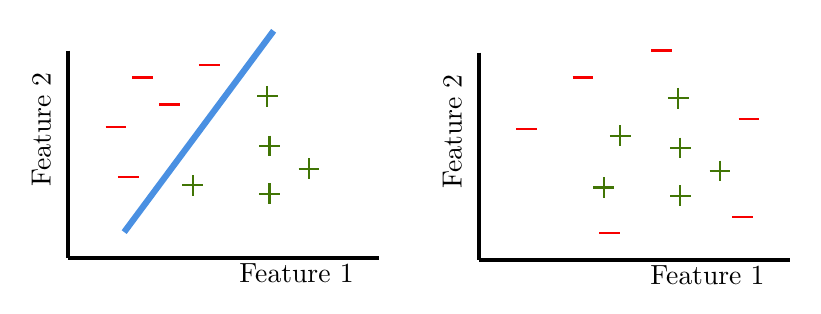
\begin{tikzpicture}[x=0.75pt,y=0.75pt,yscale=-1,xscale=1]
%uncomment if require: \path (0,300); %set diagram left start at 0, and has height of 300

%Straight Lines [id:da34928766651876697] 
\draw [line width=1.5]    (40,220) -- (190,220) ;
%Straight Lines [id:da5068123062544778] 
\draw [line width=1.5]    (40,120) -- (40,220) ;
%Straight Lines [id:da02959929373017789] 
\draw [color={rgb, 255:red, 247; green, 0; blue, 0 }  ,draw opacity=1 ]   (71,133) -- (81,133) ;
%Straight Lines [id:da023175201693992564] 
\draw [color={rgb, 255:red, 65; green, 117; blue, 5 }  ,draw opacity=1 ]   (132,166) -- (142,166) ;
%Straight Lines [id:da12599178724449778] 
\draw [color={rgb, 255:red, 65; green, 117; blue, 5 }  ,draw opacity=1 ]   (137,161) -- (137,171) ;

%Straight Lines [id:da014209875608111044] 
\draw [color={rgb, 255:red, 65; green, 117; blue, 5 }  ,draw opacity=1 ]   (95,185) -- (105,185) ;
%Straight Lines [id:da8046955093022794] 
\draw [color={rgb, 255:red, 65; green, 117; blue, 5 }  ,draw opacity=1 ]   (100,180) -- (100,190) ;

%Straight Lines [id:da8257858393303268] 
\draw [color={rgb, 255:red, 65; green, 117; blue, 5 }  ,draw opacity=1 ]   (151,177) -- (161,177) ;
%Straight Lines [id:da9904899777355851] 
\draw [color={rgb, 255:red, 65; green, 117; blue, 5 }  ,draw opacity=1 ]   (156,172) -- (156,182) ;

%Straight Lines [id:da4558392192767111] 
\draw [color={rgb, 255:red, 65; green, 117; blue, 5 }  ,draw opacity=1 ]   (132,189) -- (142,189) ;
%Straight Lines [id:da6277106773918533] 
\draw [color={rgb, 255:red, 65; green, 117; blue, 5 }  ,draw opacity=1 ]   (137,184) -- (137,194) ;

%Straight Lines [id:da6088809310233947] 
\draw [color={rgb, 255:red, 65; green, 117; blue, 5 }  ,draw opacity=1 ]   (131,142) -- (141,142) ;
%Straight Lines [id:da9717175839575936] 
\draw [color={rgb, 255:red, 65; green, 117; blue, 5 }  ,draw opacity=1 ]   (136,137) -- (136,147) ;

%Straight Lines [id:da05579332834233042] 
\draw [color={rgb, 255:red, 247; green, 0; blue, 0 }  ,draw opacity=1 ]   (84,146) -- (94,146) ;
%Straight Lines [id:da9339907902154778] 
\draw [color={rgb, 255:red, 247; green, 0; blue, 0 }  ,draw opacity=1 ]   (64,181) -- (74,181) ;
%Straight Lines [id:da801343700133325] 
\draw [color={rgb, 255:red, 247; green, 0; blue, 0 }  ,draw opacity=1 ]   (103,127) -- (113,127) ;
%Straight Lines [id:da6207217857469742] 
\draw [color={rgb, 255:red, 247; green, 0; blue, 0 }  ,draw opacity=1 ]   (58,157) -- (68,157) ;

%Straight Lines [id:da9774802467048496] 
\draw [line width=1.5]    (238,221) -- (388,221) ;
%Straight Lines [id:da8926029470752344] 
\draw [line width=1.5]    (238,121) -- (238,221) ;
%Straight Lines [id:da391932663930169] 
\draw [color={rgb, 255:red, 247; green, 0; blue, 0 }  ,draw opacity=1 ]   (360,200) -- (370,200) ;
%Straight Lines [id:da45698367355392255] 
\draw [color={rgb, 255:red, 65; green, 117; blue, 5 }  ,draw opacity=1 ]   (330,167) -- (340,167) ;
%Straight Lines [id:da8509197980874896] 
\draw [color={rgb, 255:red, 65; green, 117; blue, 5 }  ,draw opacity=1 ]   (335,162) -- (335,172) ;

%Straight Lines [id:da46487388742354385] 
\draw [color={rgb, 255:red, 65; green, 117; blue, 5 }  ,draw opacity=1 ]   (293,186) -- (303,186) ;
%Straight Lines [id:da6402947556346299] 
\draw [color={rgb, 255:red, 65; green, 117; blue, 5 }  ,draw opacity=1 ]   (298,181) -- (298,191) ;

%Straight Lines [id:da371430190479477] 
\draw [color={rgb, 255:red, 65; green, 117; blue, 5 }  ,draw opacity=1 ]   (349,178) -- (359,178) ;
%Straight Lines [id:da029152498087926304] 
\draw [color={rgb, 255:red, 65; green, 117; blue, 5 }  ,draw opacity=1 ]   (354,173) -- (354,183) ;

%Straight Lines [id:da7641303373625803] 
\draw [color={rgb, 255:red, 65; green, 117; blue, 5 }  ,draw opacity=1 ]   (330,190) -- (340,190) ;
%Straight Lines [id:da8503441823041022] 
\draw [color={rgb, 255:red, 65; green, 117; blue, 5 }  ,draw opacity=1 ]   (335,185) -- (335,195) ;

%Straight Lines [id:da14090483844456858] 
\draw [color={rgb, 255:red, 65; green, 117; blue, 5 }  ,draw opacity=1 ]   (329,143) -- (339,143) ;
%Straight Lines [id:da10211881619757635] 
\draw [color={rgb, 255:red, 65; green, 117; blue, 5 }  ,draw opacity=1 ]   (334,138) -- (334,148) ;

%Straight Lines [id:da8074255152632699] 
\draw [color={rgb, 255:red, 247; green, 0; blue, 0 }  ,draw opacity=1 ]   (296,208) -- (306,208) ;
%Straight Lines [id:da01705778265856206] 
\draw [color={rgb, 255:red, 247; green, 0; blue, 0 }  ,draw opacity=1 ]   (363,153) -- (373,153) ;
%Straight Lines [id:da4845113413868791] 
\draw [color={rgb, 255:red, 247; green, 0; blue, 0 }  ,draw opacity=1 ]   (283,133) -- (293,133) ;
%Straight Lines [id:da861487465385409] 
\draw [color={rgb, 255:red, 247; green, 0; blue, 0 }  ,draw opacity=1 ]   (256,158) -- (266,158) ;
%Straight Lines [id:da9913185077125697] 
\draw [color={rgb, 255:red, 247; green, 0; blue, 0 }  ,draw opacity=1 ]   (321,120) -- (331,120) ;
%Straight Lines [id:da016655837516902583] 
\draw [color={rgb, 255:red, 65; green, 117; blue, 5 }  ,draw opacity=1 ]   (301,161) -- (311,161) ;
%Straight Lines [id:da48554389877316395] 
\draw [color={rgb, 255:red, 65; green, 117; blue, 5 }  ,draw opacity=1 ]   (306,156) -- (306,166) ;


%Straight Lines [id:da7796305041163321] 
\draw [color={rgb, 255:red, 74; green, 144; blue, 226 }  ,draw opacity=1 ][line width=2.25]    (139,110.5) -- (67,207.5) ;

% Text Node
\draw (319,222) node [anchor=north west][inner sep=0.75pt]   [align=left] {Feature 1};
% Text Node
\draw (219,188) node [anchor=north west][inner sep=0.75pt]  [rotate=-270] [align=left] {Feature 2};
% Text Node
\draw (121,221) node [anchor=north west][inner sep=0.75pt]   [align=left] {Feature 1};
% Text Node
\draw (21,187) node [anchor=north west][inner sep=0.75pt]  [rotate=-270] [align=left] {Feature 2};


\end{tikzpicture}
\caption[Linear separability]{Linearly separable classes on the left and non-linearly separable classes on the right. Two classes are linearly separable if there exists a hyperplane for which all examples of one class are on the same side of this hyperplane, whilst all examples of the other class are on the other side of the hyperplane. In two dimensions, the hyperplane is a straight line.}
\label{fig:linear_separability}
\end{figure}

\begin{figure}
\centering
\tikzset{every picture/.style={line width=0.75pt}} %set default line width to 0.75pt        
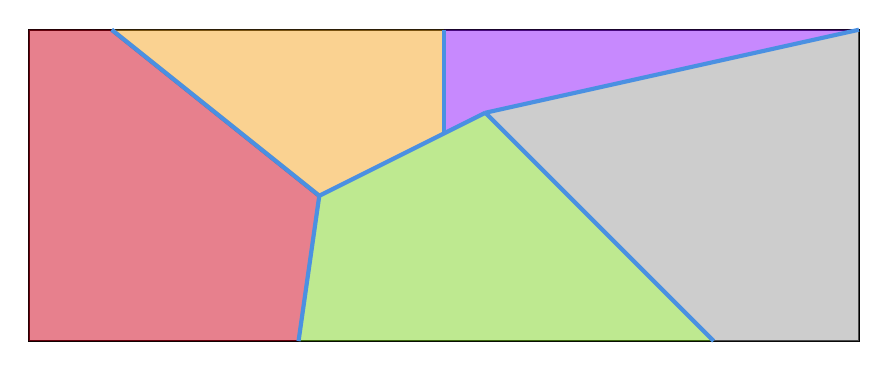
\begin{tikzpicture}[x=0.75pt,y=0.75pt,yscale=-1,xscale=1]
%uncomment if require: \path (0,300); %set diagram left start at 0, and has height of 300

%Shape: Rectangle [id:dp93531352845845] 
\draw   (10,10) -- (410,10) -- (410,160) -- (10,160) -- cycle ;
%Straight Lines [id:da6152066863993235] 
\draw [color={rgb, 255:red, 74; green, 144; blue, 226 }  ,draw opacity=1 ][line width=1.5]    (50,10) -- (150,90) ;
%Shape: Polygon [id:ds7775874145177377] 
\draw  [draw opacity=0][fill={rgb, 255:red, 208; green, 2; blue, 27 }  ,fill opacity=0.5 ] (10,10) -- (50,10) -- (150,90) -- (140,160) -- (10,160) -- cycle ;
%Shape: Polygon [id:ds9784233202991128] 
\draw  [draw opacity=0][fill={rgb, 255:red, 245; green, 166; blue, 35 }  ,fill opacity=0.5 ] (50,10) -- (210,10) -- (210,60) -- (150,90) -- cycle ;
%Straight Lines [id:da46278066568077114] 
\draw [color={rgb, 255:red, 74; green, 144; blue, 226 }  ,draw opacity=1 ][line width=1.5]    (50,10) -- (150,90) ;
%Shape: Polygon [id:ds26003561212820947] 
\draw  [draw opacity=0][fill={rgb, 255:red, 126; green, 211; blue, 33 }  ,fill opacity=0.5 ] (150,90) -- (230,50) -- (340,160) -- (140,160) -- cycle ;
%Shape: Polygon [id:ds9559236222145457] 
\draw  [draw opacity=0][fill={rgb, 255:red, 144; green, 19; blue, 254 }  ,fill opacity=0.5 ] (210,60) -- (230,50) -- (410,10) -- (210,10) -- cycle ;
%Shape: Polygon [id:ds03375440764371551] 
\draw  [draw opacity=0][fill={rgb, 255:red, 155; green, 155; blue, 155 }  ,fill opacity=0.5 ] (230,50) -- (410,10) -- (410,120) -- (410,160) -- (340,160) -- cycle ;
%Straight Lines [id:da4209706928929018] 
\draw [color={rgb, 255:red, 74; green, 144; blue, 226 }  ,draw opacity=1 ][line width=1.5]    (150,90) -- (140,160) ;
%Straight Lines [id:da8034752362025392] 
\draw [color={rgb, 255:red, 74; green, 144; blue, 226 }  ,draw opacity=1 ][line width=1.5]    (150,90) -- (230,50) ;
%Straight Lines [id:da8987706587716273] 
\draw [color={rgb, 255:red, 74; green, 144; blue, 226 }  ,draw opacity=1 ][line width=1.5]    (210,10) -- (210,60) ;
%Straight Lines [id:da07108977100440117] 
\draw [color={rgb, 255:red, 74; green, 144; blue, 226 }  ,draw opacity=1 ][line width=1.5]    (230,50) -- (410,10) ;
%Straight Lines [id:da5244033806754336] 
\draw [color={rgb, 255:red, 74; green, 144; blue, 226 }  ,draw opacity=1 ][line width=1.5]    (230,50) -- (340,160) ;
\end{tikzpicture}
\caption[Decision boundaries and decision regions]{Decision boundaries (blue lines) separate different decision regions (colored regions).}
\label{fig:decision_boundaries_decision_regions}
\end{figure}

\begin{figure}
\centering
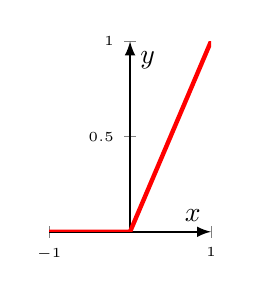
\begin{tikzpicture}
\begin{axis}[width=0.30\textwidth,
height=4cm,
axis lines=middle,
xlabel=$x$,
ylabel=$y$,
xmin=-1,
xmax=1,
ymin=0,
ymax=1,
xtick={-1,1},
ytick={0,0.5,1},
axis line style={-latex},
ticklabel style={font=\tiny,fill=white},
]
\addplot[ultra thick, color=red]{max(0,x)};
\end{axis}
\end{tikzpicture}
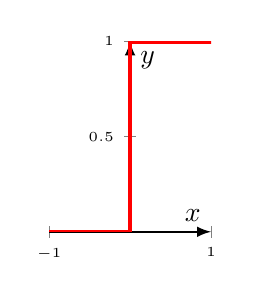
\begin{tikzpicture}
\begin{axis}[width=0.30\textwidth,
height=4cm,
axis lines=middle,
xlabel=$x$,
ylabel=$y$,
xmin=-1,
xmax=1,
ymin=0,
ymax=1,
xtick={-1,1},
ytick={0,0.5,1},
axis line style={-latex},
ticklabel style={font=\tiny,fill=white},
]
\addplot+[const plot, no marks, ultra thick, color=red] coordinates {(-10,0) (0,1) (10, 1)};
\end{axis}
\end{tikzpicture}
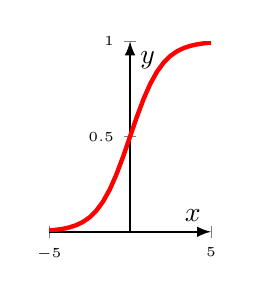
\begin{tikzpicture}
\begin{axis}[width=0.30\textwidth,
height=4cm,
axis lines=middle,
xlabel=$x$,
ylabel=$y$,
xmin=-5,
xmax=5,
ymin=0,
ymax=1,
xtick={-5,5},
ytick={0,0.5,1},
axis line style={-latex},
ticklabel style={font=\tiny,fill=white},
]
\addplot[ultra thick, color=red]{exp(x) / (1 + exp(x))};
\end{axis}
\end{tikzpicture}
\caption[Activiation functions]{Plots of different activation functions. From left to right: \gls{relu}, Heaviside step and sigmoid.}
\label{fig:activation_functions}
\end{figure}

\section{Adversarial attacks}
The expressiveness of \glspl{ann} is a double-edged sword. It is the cause for the near-human performance on some tasks, but also for counter-intuitive properties. As studied by Szegedy et al \cite{szegedy2014intriguing}, one of these properties is the presence of discontinuous decision boundaries. This might cause seemingly identically images to be classified differently. They first defined adversarial examples as \textit{imperceptibly small perturbations to a correctly classified input image, so that it is no longer classified correctly} \cite{szegedy2014intriguing}. This property of \glspl{ann} might not seem important at first glance, but it can be quite worrisome from a security point-of-view. Malicious users could craft images to bypass face recognition software \cite{face_recognition} or attack the camera of a self-driving car to misclassify traffic signs \cite{traffic_signs}. Other fields where adversarial examples are of interest include malware detection \cite{malware_detection}, natural language processing \cite{adversarial_nlp} and industrial control systems \cite{adversarial_industrial_control_system}. Adversarial attacks are algorithms used to craft such adversarial examples.\\ 

Most research on adversarial attacks is done using images. Researchers have the most freedom in this domain, since a slightly altered image is still an image with roughly the same contents. Slightly modifying an industrial control system however, might break the entire way the system works. Research in other domains is mostly conducted by altering existing image algorithms to the specific use case. For this reason this works only focuses on adversarial attacks on images.\\ 

\subsection{Adversarial attacks terminology}
Adversarial attacks are generally divided in two categories, white box attacks and black box attacks. In a white box attack, the attacker has complete knowledge of the classifier under attack. This knowledge consists of the architecture, parameters and thus their gradients and all output of the classifier. Examples of white box attacks are the \gls{fgsm} \cite{FGSM} or the Carlini \& Wagner attack \cite{cw_attack}.\\

In black box attacks, the only thing the attacker has access to is the output of the model. Depending on the literature, this output consists of class labels only (decision-based attack) or class labels and the corresponding confidence scores (score-based attacks). Black box attacks are more relevant in real-life scenarios, since most attacks are performed on a third-party \gls{api}. These \glspl{api} generally do not reveal the underlying model.\\

Both white box and black box attacks can be divided into targeted and untargeted attacks depending on their goal. In a targeted attack, the goal of the attacker is to create an adversarial example with a specific target class. In an untargeted attack the target class can be any class. Untargeted variants of attacks generally enjoy much more freedom and are therefore able to craft adversarial examples that are closer to the original. Figure \ref{fig:target_vs_untargeted} visually explains the difference between the two types.\\

\begin{figure}
\centering
\tikzset{every picture/.style={line width=0.75pt}} %set default line width to 0.75pt        
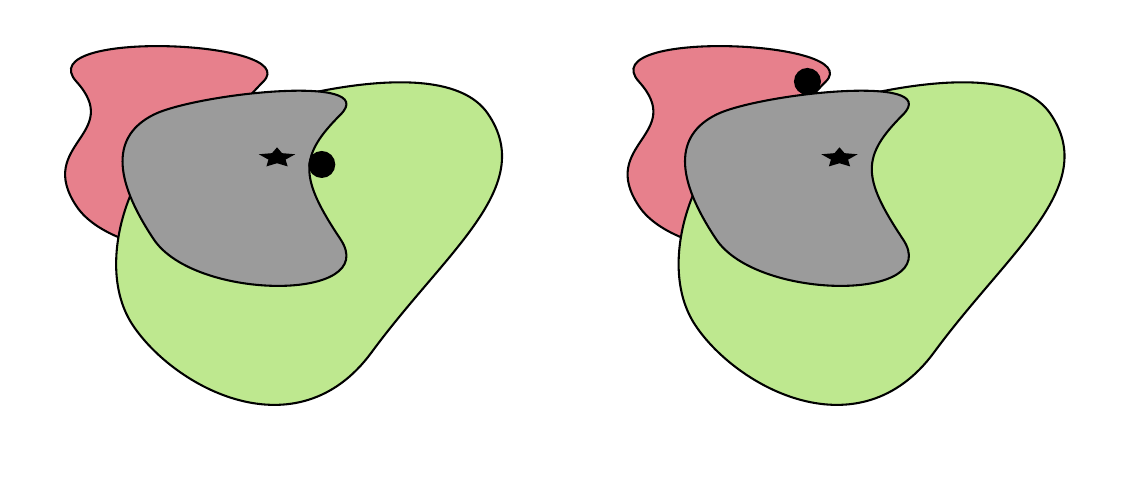
\begin{tikzpicture}[x=0.75pt,y=0.75pt,yscale=-1,xscale=1]
%uncomment if require: \path (0,300); %set diagram left start at 0, and has height of 300

%Shape: Polygon Curved [id:ds8186148148213988] 
\draw  [fill={rgb, 255:red, 231; green, 128; blue, 140 }  ,fill opacity=1 ] (288.8,37.12) .. controls (265.8,11.62) and (398.8,17.12) .. (378.8,37.12) .. controls (358.8,57.12) and (358.8,67.12) .. (378.8,97.12) .. controls (398.8,127.12) and (308.8,127.12) .. (288.8,97.12) .. controls (268.8,67.12) and (311.8,62.62) .. (288.8,37.12) -- cycle ;
%Shape: Polygon Curved [id:ds7649136964229322] 
\draw  [fill={rgb, 255:red, 190; green, 232; blue, 143 }  ,fill opacity=1 ] (337,63.03) .. controls (357,53.03) and (463,17.53) .. (487,52.53) .. controls (511,87.53) and (467,118.53) .. (431,167.53) .. controls (395,216.53) and (336,184.53) .. (316,154.53) .. controls (296,124.53) and (317,73.03) .. (337,63.03) -- cycle ;
%Shape: Polygon Curved [id:ds811213596684691] 
\draw  [fill={rgb, 255:red, 155; green, 155; blue, 155 }  ,fill opacity=1 ] (326,53.03) .. controls (346,43.03) and (436,33.03) .. (416,53.03) .. controls (396,73.03) and (396,83.03) .. (416,113.03) .. controls (436,143.03) and (346,143.03) .. (326,113.03) .. controls (306,83.03) and (306,63.03) .. (326,53.03) -- cycle ;

%Shape: Star [id:dp7949967265036502] 
\draw  [fill={rgb, 255:red, 0; green, 0; blue, 0 }  ,fill opacity=1 ] (385.44,69.53) -- (387.62,72.06) -- (392.51,72.47) -- (388.97,74.44) -- (389.81,77.22) -- (385.44,75.91) -- (381.07,77.22) -- (381.9,74.44) -- (378.36,72.47) -- (383.25,72.06) -- cycle ;

%Shape: Circle [id:dp639830751531604] 
\draw  [fill={rgb, 255:red, 0; green, 0; blue, 0 }  ,fill opacity=1 ] (364,37.03) .. controls (364,33.72) and (366.69,31.03) .. (370,31.03) .. controls (373.31,31.03) and (376,33.72) .. (376,37.03) .. controls (376,40.35) and (373.31,43.03) .. (370,43.03) .. controls (366.69,43.03) and (364,40.35) .. (364,37.03) -- cycle ;
%Shape: Polygon Curved [id:ds526086534908093] 
\draw  [fill={rgb, 255:red, 231; green, 128; blue, 140 }  ,fill opacity=1 ] (17.8,37.12) .. controls (-5.2,11.62) and (127.8,17.12) .. (107.8,37.12) .. controls (87.8,57.12) and (87.8,67.12) .. (107.8,97.12) .. controls (127.8,127.12) and (37.8,127.12) .. (17.8,97.12) .. controls (-2.2,67.12) and (40.8,62.62) .. (17.8,37.12) -- cycle ;
%Shape: Polygon Curved [id:ds40487542108345687] 
\draw  [fill={rgb, 255:red, 190; green, 232; blue, 143 }  ,fill opacity=1 ] (66,63.03) .. controls (86,53.03) and (192,17.53) .. (216,52.53) .. controls (240,87.53) and (196,118.53) .. (160,167.53) .. controls (124,216.53) and (65,184.53) .. (45,154.53) .. controls (25,124.53) and (46,73.03) .. (66,63.03) -- cycle ;
%Shape: Polygon Curved [id:ds8878674517678289] 
\draw  [fill={rgb, 255:red, 155; green, 155; blue, 155 }  ,fill opacity=1 ] (55,53.03) .. controls (75,43.03) and (165,33.03) .. (145,53.03) .. controls (125,73.03) and (125,83.03) .. (145,113.03) .. controls (165,143.03) and (75,143.03) .. (55,113.03) .. controls (35,83.03) and (35,63.03) .. (55,53.03) -- cycle ;

%Shape: Star [id:dp9101553466481458] 
\draw  [fill={rgb, 255:red, 0; green, 0; blue, 0 }  ,fill opacity=1 ] (114.44,69.53) -- (116.62,72.06) -- (121.51,72.47) -- (117.97,74.44) -- (118.81,77.22) -- (114.44,75.91) -- (110.07,77.22) -- (110.9,74.44) -- (107.36,72.47) -- (112.25,72.06) -- cycle ;

%Shape: Circle [id:dp29014472584929707] 
\draw  [fill={rgb, 255:red, 0; green, 0; blue, 0 }  ,fill opacity=1 ] (130,77.03) .. controls (130,73.72) and (132.69,71.03) .. (136,71.03) .. controls (139.31,71.03) and (142,73.72) .. (142,77.03) .. controls (142,80.35) and (139.31,83.03) .. (136,83.03) .. controls (132.69,83.03) and (130,80.35) .. (130,77.03) -- cycle ;
\end{tikzpicture}
\caption[Difference targeted and untargeted attack]{Different decision regions are shown in different colors. An adversarial example is being created starting from the source image (black star). On the left an untargeted attack is performed. The adversarial example is the image closest to the source image, that is classified differently (black circle). On the right a targeted attack is performed with the red decision region being the target class. The adversarial example is the image closest to the source image that is in the red decision region.}
\label{fig:target_vs_untargeted}
\end{figure}

What does it mean for images to be close to each other? This is easy to visualize in two dimensions as in Figure \ref{fig:target_vs_untargeted}, but in higher dimensions, this is more difficult. Images reside in $d$-dimensional space, where $d$ is the amount of pixels of the image. Two commonly used distances in higher dimensions are the $L_2$-distance and the $L_\infty$-distance. They are defined as follows:

\begin{align*}
L_2(X, Y) &= \sqrt{\sum_{i=1}^d|x_i - y_i|^2} \\
L_\infty(X, Y) &= \lim_{p\rightarrow \infty}\left( \sum_{i=1}^d|x_i-y_i|^p\right)^{1/p} \\
&= \max (|x_1 - y_1|, |x_2-y_2|, \ldots, |x_d-y_d|)
\end{align*}

In both distances $X$ and $Y$ represent the images and $(x_1, x_2, \ldots, x_i, \ldots, x_d)$ and $(y_1, y_2, \ldots, y_i, \ldots, y_d)$ are the pixel values of $X$ and $Y$ respectively. The $L_2$-distance is also known as the Euclidean distance, which is a generalization of the Pythagorean theorem in more than two dimensions. It takes the pairwise distances between all pixels into account. The $L_\infty$-distance is also called the Chebyshev distance. This distance only depends on the maximal pairwise distance between the two images. By minimizing the $L_\infty$-distance, the maximal pixelwise difference in minimized \cite{wiki_distances}. 

\subsection{Adversarial defenses}

\section{Particle swarm optimization}
\gls{pso} \cite{pso} is an optimization framework part of the \glspl{ea} family. In \glspl{ea}, populations of candidate solutions evolve based on mechanisms inspired by the field op biology, such as ant colonies \cite{aco}, mutation and recombination \cite{genetic_algorithm}. The mechanism that inspired \gls{pso} is the flocking of birds. The framework has been applied to numerous problems such as routing problems \cite{ev_transport, freight_transport}, diagnosing diseases from imaging \cite{leukemia_pso} and calculating heat transfer coefficients \cite{heat_transfer_pso}.\\

In \gls{pso}, different particles move through the search space based on a set of rules. Each position in the search space has a given fitness value. This value determines how 'fit' or good a certain position is with respect to the goal of the optimization problem. Every iteration, all particles take a step towards their personal best position, towards the group or swarm's best position and a step in the current direction (inertia). The different step sizes can be weighted depending on the problem at hand. In Figure \ref{fig:pso}, the steps are graphically represented for a single particle.   

\begin{figure}
\centering
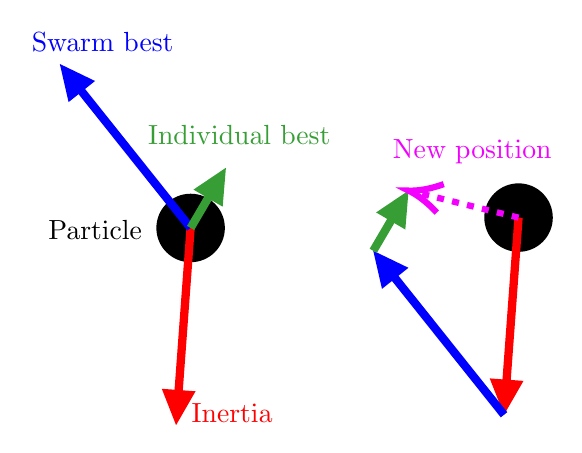
\begin{tikzpicture}[x=0.75pt,y=0.75pt,yscale=-1,xscale=1]

%uncomment if require: \path (0,300); %set diagram left start at 0, and has height of 300

%Shape: Circle [id:dp06935534605548432] 
\draw  [fill={rgb, 255:red, 0; green, 0; blue, 0 }  ,fill opacity=1 ] (100,161) .. controls (100,152.16) and (107.16,145) .. (116,145) .. controls (124.84,145) and (132,152.16) .. (132,161) .. controls (132,169.84) and (124.84,177) .. (116,177) .. controls (107.16,177) and (100,169.84) .. (100,161) -- cycle ;
%Straight Lines [id:da36297070749556615] 
\draw [color={rgb, 255:red, 255; green, 0; blue, 0 }  ,draw opacity=1 ][line width=3]    (116,161) -- (109.44,250.02) ;
\draw [shift={(109,256)}, rotate = 274.21] [fill={rgb, 255:red, 255; green, 0; blue, 0 }  ,fill opacity=1 ][line width=0.08]  [draw opacity=0] (16.97,-8.15) -- (0,0) -- (16.97,8.15) -- cycle    ;
%Shape: Circle [id:dp2975589876543052] 
\draw  [fill={rgb, 255:red, 0; green, 0; blue, 0 }  ,fill opacity=1 ] (258,156) .. controls (258,147.16) and (265.16,140) .. (274,140) .. controls (282.84,140) and (290,147.16) .. (290,156) .. controls (290,164.84) and (282.84,172) .. (274,172) .. controls (265.16,172) and (258,164.84) .. (258,156) -- cycle ;
%Straight Lines [id:da11974704599725938] 
\draw [color={rgb, 255:red, 255; green, 0; blue, 0 }  ,draw opacity=1 ][line width=3]    (274,156) -- (267.44,245.02) ;
\draw [shift={(267,251)}, rotate = 274.21] [fill={rgb, 255:red, 255; green, 0; blue, 0 }  ,fill opacity=1 ][line width=0.08]  [draw opacity=0] (16.97,-8.15) -- (0,0) -- (16.97,8.15) -- cycle    ;
%Straight Lines [id:da34669530870861953] 
\draw [color={rgb, 255:red, 0; green, 0; blue, 255 }  ,draw opacity=1 ][line width=3]    (267,251) -- (207.74,176.69) ;
\draw [shift={(204,172)}, rotate = 51.43] [fill={rgb, 255:red, 0; green, 0; blue, 255 }  ,fill opacity=1 ][line width=0.08]  [draw opacity=0] (16.97,-8.15) -- (0,0) -- (16.97,8.15) -- cycle    ;
%Straight Lines [id:da2944239439562262] 
\draw [color={rgb, 255:red, 55; green, 158; blue, 54 }  ,draw opacity=1 ][line width=3]    (204,172) -- (217.97,148.18) ;
\draw [shift={(221,143)}, rotate = 120.38] [fill={rgb, 255:red, 55; green, 158; blue, 54 }  ,fill opacity=1 ][line width=0.08]  [draw opacity=0] (16.97,-8.15) -- (0,0) -- (16.97,8.15) -- cycle    ;
%Straight Lines [id:da9472051718664152] 
\draw [color={rgb, 255:red, 243; green, 0; blue, 255 }  ,draw opacity=1 ][line width=2.25]  [dash pattern={on 2.53pt off 3.02pt}]  (274,156) -- (224.88,143.95) ;
\draw [shift={(221,143)}, rotate = 13.78] [color={rgb, 255:red, 243; green, 0; blue, 255 }  ,draw opacity=1 ][line width=2.25]    (15.74,-7.06) .. controls (10.01,-3.31) and (4.76,-0.96) .. (0,0) .. controls (4.76,0.96) and (10.01,3.31) .. (15.74,7.06)   ;
%Straight Lines [id:da8503925276289086] 
\draw [color={rgb, 255:red, 0; green, 0; blue, 255 }  ,draw opacity=1 ][line width=3]    (116,161) -- (56.74,86.69) ;
\draw [shift={(53,82)}, rotate = 51.43] [fill={rgb, 255:red, 0; green, 0; blue, 255 }  ,fill opacity=1 ][line width=0.08]  [draw opacity=0] (16.97,-8.15) -- (0,0) -- (16.97,8.15) -- cycle    ;
%Straight Lines [id:da10251717157021911] 
\draw [color={rgb, 255:red, 55; green, 158; blue, 54 }  ,draw opacity=1 ][line width=3]    (116,161) -- (129.97,137.18) ;
\draw [shift={(133,132)}, rotate = 120.38] [fill={rgb, 255:red, 55; green, 158; blue, 54 }  ,fill opacity=1 ][line width=0.08]  [draw opacity=0] (16.97,-8.15) -- (0,0) -- (16.97,8.15) -- cycle    ;

% Text Node
\draw (46,156) node [anchor=north west][inner sep=0.75pt]   [align=left] {Particle};
% Text Node
\draw (115,244) node [anchor=north west][inner sep=0.75pt]   [align=left] {\textcolor[rgb]{1,0,0}{Inertia}};
% Text Node
\draw (38,65) node [anchor=north west][inner sep=0.75pt]  [color={rgb, 255:red, 0; green, 0; blue, 255 }  ,opacity=1 ] [align=left] {Swarm best};
% Text Node
\draw (94,110) node [anchor=north west][inner sep=0.75pt]  [color={rgb, 255:red, 55; green, 158; blue, 54 }  ,opacity=1 ] [align=left] {Individual best};
% Text Node
\draw (212,117) node [anchor=north west][inner sep=0.75pt]   [align=left] {\textcolor[rgb]{0.95,0,1}{New position}};


\end{tikzpicture}
\caption[Particle swarm optimization]{Particles move based on a step towards their best known position, the swarm's best known position and a step in the direction of the movement of the previous iteration. The different steps are combined to determine the new position of the particle.}
\label{fig:pso}
\end{figure}
